\scanpage{55}
A) \uline{$2$ inv.}
\deleted{$g(\lambda,\mu)=0$ identiquement}
\deleted{Alors $f(\lambda s_0+\mu\widetilde o)=0\quad\forall\lambda,\mu$
sss $\sigma'$.}

Alors, indépendamment de la parité de $n$, on peut écrire
$g(\lambda,\mu)=-\sigma\mu(\lambda+\frac{\rho}{2}\mu)$,
et les équivalences décrites dans $1^\circ)$ sont valables,
avec $\rho'$ remplacé par $\rho/2$.
Les solutions de $g(\lambda,\mu)=0$, avec $\mu$ inv.,
sont multiples de $(-\frac{\rho}{2},1)$ et correspondent à
\[
-\frac{\rho}{2}s_0+\widetilde o
\]
ou encore \deleted{$\unsure{-\rho s_0+o}$}
(si $\rho$ inv. i.e. $\uline a$ défini)
\[
-s_0+2\frac{\widetilde o}{\rho}=o'-s_0=\uline a s_0
\]
\deleted{b) $S$ de car. $2$}

B) $2\,1_S=0$ i.e. $S$ de car. $2$.
On trouve alors \deleted{$f(\lambda s_0+\mu\widetilde o)$}
\[
g(\lambda,\mu)=f(\lambda s_0+\mu\widetilde o)
=\unsure{+|-}(\sigma'\rho')\mu^2
\]
c'est $\equiv0$ sss $\sigma'\rho'=0$.

c'est $\neq0$ en tt fibre sss $\sigma'\rho'$ inv.
i.e. $\sigma'$ \uline{et $\rho'$} inv.
i.e. $\sigma'$ inv. et $\uline a$ défini
(c'est le cas si $(\mathcal E,V,f)$ birégulier).
\deleted{\unsure{Cela}} Ceci signifie aussi
$D_0\not\subset Q_X$ en tt fibre, et \unsure{implique} que
$D_0$ est tangente à $Q_X$.
\margin{\[
\uline a x=x+o'=x
\]
\deleted{$f(x+o')=f(x)+f(o')+\langle x,\Psi(o')\rangle$}
car \unsure{$\sigma$ inv.} $\rho=\rho'$, \unsure{$S$}}
\figure{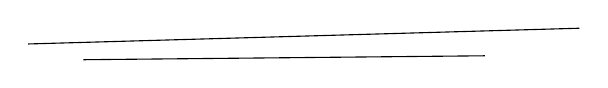
\begin{tikzpicture}
\draw (0,.2)--(7,.4);\draw (.7,0)--(5.8,.05);
\end{tikzpicture}}

\deleted{Supposons $n$ pair, $n=2m$. On s'intéresse aux systèmes
$(X,\tau_*=(\tau_i)_{0\leq i\leq n},s_0)$
\deleted{tels} non dégénérés, et tels que $\sigma(=\sigma')$ soit inv.
[Si on suppose déjà les $\beta_i$ $(0\leq i\leq n-1)$ inv.,
cela signifie $f_{\mathcal E}$ lisse.]
\deleted{Ceci définit donc}
Ceci définit donc $(X,\underbrace{Q_X}_{\text{quadrique}},\tau_*^X)$,
où maintenant les $\tau_i$ \inserted{$(0\leq i\leq n)$}
sont des autom. \unsure{involutifs} de $(X,Q_X)$.
Considérons le \unsure{antidual|multidual}:
\[
(C,Q_C,\tau_*^C)\mathbin{-}
\]
}
\mspage{54}

